
%%%%%%%%%%%%%%%%%%%%%%%%%%%%%%%%%%%%%%%%%%%%%%%%%%%%%%%%%%%%%%%%%%%%%%%%%
%%%%%%%%%%%%%%%%%%%%%%%%%%%%%%%%%%%%%%%%%%%%%%%%%%%%%%%%%%%%%%%%%%%%%%%%%
%
% A general method to find special functions that interpolate Appell polynomials,
% with examples,
% by
% A. Gil Asensi and J. L. Varona
%
% Date of last modification: 2023-09-17
%
%%%%%%%%%%%%%%%%%%%%%%%%%%%%%%%%%%%%%%%%%%%%%%%%%%%%%%%%%%%%%%%%%%%%%%%%%
%%%%%%%%%%%%%%%%%%%%%%%%%%%%%%%%%%%%%%%%%%%%%%%%%%%%%%%%%%%%%%%%%%%%%%%%%

%% ORCID:
%% J. L. Varona: 0000-0002-2023-9946
%% A. Gil Asensi: 0009-0007-9667-0744


\documentclass[11pt,a4paper]{amsart}

%\usepackage{amssymb}

%%% \allowdisplaybreaks is a command from amsmath that allow page breaks
%%% inside a multi-line formula (align, multline, gather, ...)
\allowdisplaybreaks[3] %%% Scale from 1 (weak allow) to 4 (complete allow).
%%% If a break can be avoided, we can use \\* instead of \\

%---------------------
\usepackage{url}
\usepackage[colorlinks,linkcolor=blue,citecolor=blue]{hyperref}
%---------------------

%%%%%%%%%%%%%%%%%%%%%%%%%%%%
%%% ONLY FOR DRAFTS:
%\usepackage[utf8]{inputenc}
%\usepackage{color}
%\newcommand{\rojo}[1]{\textcolor{red}{#1}}
%\newcommand{\azul}[1]{\textcolor{blue}{#1}}
%\newcommand{\verde}[1]{\textcolor{green}{#1}}
%%%%%%%%%%%%%%%%%%%%%%%%%%%%

%---------------------
%\usepackage{graphicx}
\usepackage{tikz}
%---------------------

%%%%%%%%%%%%%%%%%%%%%%%%%%%%
%% ONLY FOR DRAFTS:
%\usepackage[notcite,notref]{showkeys}
%\usepackage{refcheck}
%\usepackage[hyperpageref]{backref} % For drafts
%\usepackage{backref}
%%%%%%%%%%%%%%%%%%%%%%%%%%%%

\usepackage[headings]{fullpage}

%---------------------
%%--- Definitions for the functions pFq.
%%--- In this way is only for 1F2 and 2F1
%%--- (for general pFq it is enough to use two extra parameters).
%%%% Version for displaymath:
%\newcommand{\FFunodos}[3]{{}_{1}F_{2}\bigg(\genfrac{}{}{0pt}{}{#1}{#2};#3\bigg)}
%\newcommand{\FFdosuno}[3]{{}_{2}F_{1}\bigg(\genfrac{}{}{0pt}{}{#1}{#2};#3\bigg)}
%% (Instead of ; we can put \,\bigg|\, if we prefer | to separate #3)
%%%% Version for text:
%\newcommand{\tFFunodos}[3]{{}_{1}F_{2}\Big(\genfrac{}{}{0pt}{}{#1}{#2};#3\Big)}
%\newcommand{\tFFdosuno}[3]{{}_{2}F_{1}\Big(\genfrac{}{}{0pt}{}{#1}{#2};#3\Big)}
%% It is also possible to define the structure only for the parenthesis, 
%% and and to add{}_{p}F_{q} at the beginning. 
%% This can also be used for the Meijer functions G_{p,q}^{m,n}:
%%%% Version for displaymath:
\newcommand{\parenG}[3]{\bigg(\genfrac{}{}{0pt}{}{#1}{#2} \,\bigg|\, #3\bigg)}
%%%% Version for text:
\newcommand{\tparenG}[3]{\Big(\genfrac{}{}{0pt}{}{#1}{#2} \,\Big|\, #3\Big)}
%---------------------

%\newcommand{\D}{\mathbb{D}}
\newcommand{\N}{\mathbb{N}}
\newcommand{\Z}{\mathbb{Z}}
\newcommand{\Q}{\mathbb{Q}}
\newcommand{\R}{\mathbb{R}}
\newcommand{\C}{\mathbb{C}}
\newcommand{\calO}{\mathcal{O}}
\newcommand{\eps}{\varepsilon}

\newcommand{\Ch}{\operatorname{Ch}}

\newcommand{\Ea}{E_{\alpha}}
\newcommand{\La}{\Lambda_{\alpha}}
%\newcommand{\Lax}{\Lambda_{\alpha,x}}
%\newcommand{\Fa}{\mathcal{F}_{\alpha}} % Dunkl transform of order \alpha
%\newcommand{\mua}{\mu_{\alpha}}
%\newcommand{\binoma}[2]{\binom{#1}{#2}_{\!\alpha}}

\renewcommand{\Re}{\operatorname{Re}}
\renewcommand{\Im}{\operatorname{Im}}

\newcommand{\Res}{\operatornamewithlimits{Res}}

%\newcommand{\Li}{\operatorname{Li}}
%\newcommand{\pochhammer}[2]{(#1)_{#2}}
%\newcommand{\factorialdown}[2]{[#1]_{#2}}

%\newcommand{\dist}{\mathop{\mathrm{dist}}}
%\newcommand{\re}{\mathop{\mathrm{Re}}}
%\newcommand{\im}{\mathop{\mathrm{Im}}}

%-----------
\theoremstyle{plain}
\newtheorem{theorem}{Theorem}[section]

%\theoremstyle{plain}
%\newtheorem{proposition}[theorem]{Proposition}

%\theoremstyle{plain}
%\newtheorem{corollary}[theorem]{Corollary}

\theoremstyle{plain}
\newtheorem{lemma}[theorem]{Lemma}

% \theoremstyle{plain}
% \newtheorem*{conjecture}{Conjecture}

% \theoremstyle{plain}
% \newtheorem{property}{Property}

%\theoremstyle{definition}
%\newtheorem{definition}[theorem]{Definition}

\theoremstyle{remark}
\newtheorem{remark}{Remark}

%\theoremstyle{remark}
%\newtheorem*{note}{Note}
%-----------

\numberwithin{equation}{section}

%-----------
\title[Special functions that interpolate Appell polynomials]%
{A general method to find special functions that interpolate Appell polynomials, 
with examples}
%-----------


%-----------
\author[A. Gil Asensi]{Alejandro Gil Asensi}
\address{%
       Departamento de Matem\'aticas y Computaci\'on,
       Universidad de La Rioja,
       26006 Logro\~no, Spain}
\email{algila@unirioja.es}

\author[J.~L.~Varona]{Juan L. Varona}
\address{%
       Departamento de Matem\'aticas y Computaci\'on,
       Universidad de La Rioja,
       26006 Logro\~no, Spain}
\email{jvarona@unirioja.es}
\urladdr{http://www.unirioja.es/cu/jvarona/}
%-----------

%\thanks{\textbf{A. Gil Asensi}, Departamento de Matem\'aticas y Computaci\'on, 
%Universidad de La Rioja,
%26006 Logro\~no, Spain, algila@unirioja.es. ORCID: 0009-0002-2023-9946}

%\thanks{\textbf{J.~L.~Varona}, Departamento de Matem\'aticas y Computaci\'on, 
%Universidad de La Rioja,
%26006 Logro\~no, Spain, jvarona@unirioja.es. ORCID: 0000-0002-2023-9946}

\renewcommand{\datename}{THIS PAPER HAS BEEN PUBLISHED IN:}
\date{\textit{J.\ Math.\ Anal.\ Appl.}\ \textbf{531} (2024), no.~2, 127825; 
DOI: \url{https://doi.org/10.1016/j.jmaa.2023.127825}}
%% Online first:
%\date{\textit{J.\ Math.\ Anal.\ Appl.}, online first October~5, 2023, 
%doi: 10.1016/j.jmaa.2023.127825.}

\thanks{This research was partially supported by PID2021-124332NB-C22 (Minis\-te\-rio de Cien\-cia e Inno\-va\-ci\'on, Spain)}

%-----------
\subjclass[2020]{Primary 11B83; Secondary 30B40, 33C60, 44A20}
\keywords{Appell sequences, special functions, Mellin transforms, truncated exponential polynomials, 
Appell-Dunkl polynomials}
%-----------

%---------------------
\begin{document}
%---------------------

%% Class amsart Warning: Abstract should precede \maketitle in AMS document class
%-----------
\begin{abstract}
Given an Appell sequence $\{P_n(x)\}_{n=0}^\infty$ defined by means of a generating function
\[
A(t) e^{xt} = \sum_{n=0}^\infty P_{n}(x)\frac{t^n}{n!},
\]
we discuss a general procedure for constructing a complex function $F(s,x)$, which is entire in $s$ for each fixed $x$ with $\operatorname{Re}x > 0$, and satisfies $F(-n,x) = P_n(x)$ at $n = 0,1,2,\dots$. The method is based on the Mellin transform and allows $A(-t)$ to have isolated singularities on the half-line $(0,\infty)$, in contrast with other general methods that appear in the mathematical literature. We illustrate our procedure with  some elucidatory examples. However, our approach cannot be used for analogously defined Appell-Dunkl sequences, a fact which has led us to include an open problem related to this case.
\end{abstract}
%-----------

%---------------------
\maketitle
%---------------------

%-----------
\section{Introduction} 
%-----------

An Appell sequence $\{P_{n}(x)\}_{n=0}^{\infty}$ is defined formally by an exponential generating function of the form
\begin{equation}
\label{E:Appell_GF}
  G(x,t) = A(t) e^{xt} = \sum_{n=0}^\infty P_{n}(x)\frac{t^n}{n!},
\end{equation}
where $x,t$ are indeterminates and $A(t)$ is a formal power series.

It is easily seen that~\eqref{E:Appell_GF} implies $P_{n}(x)$ is a polynomial of the form
\begin{equation*}
  P_{n}(x) = A(0)x^n+\cdots.
\end{equation*}
Thus, the assumption $A(0) \neq 0$ (which is usually given together with~\eqref{E:Appell_GF}) means that $P_{n}(x)$ has degree~$n$.
In addition, it is straightforward to verify that any such generating function has polynomial coefficients satisfying $P_{n}'(x) = n P_{n-1}(x)$ for all $n \geq 1$, and conversely, that this condition on a polynomial sequence is equivalent to having a generating function of the given form. 
 
The members of an Appell sequence are called Appell polynomials. Typical examples of Appell sequences are the Bernoulli, Euler, and Hermite polynomials, whose generating functions $G(x,t)$ are respectively $te^{xt}/(e^t-1)$, $2e^{xt}/(e^t+1)$ and $e^{-t^2/2}$.

In a series of recent papers \cite{NRV, NRV2, NRV3}, the authors give a method to build transcendental functions whose values at the negative integers are the polynomials defined by~\eqref{E:Appell_GF}, requiring only a few easy conditions on the function $A(t)$, and provide many examples and properties. This method uses a slight modification of the Mellin transform of the generating function $G(x,-t)$ (note the sign change) and conditions on $A(t)$ that ensure the integral defining the transform converges. For instance, for the Bernoulli polynomials $\{B_n(x)\}_{n=0}^{\infty}$ the corresponding function is $s\zeta(s+1,x)$, where $\zeta(s,x)$ is the Hurwitz zeta function. This is not surprising, since a well-known property of $\zeta(s,x)$ is $\zeta(-n+1,x) = -B_{n}(x)/n$. Many other examples, such as those coming from some generalizations of the Bernoulli and Euler polynomials, the classical Hermite and Laguerre polynomials, and the Bell numbers, are discussed there.

However, although the conditions on $A(t)$ given in~\cite{NRV} are rather general, one of them requires that $A(-t)$ be continuous on $[0, +\infty)$, thus excluding complex analytic functions $A(-t)$ with singularities on $(0, +\infty)$; indeed, the Mellin transform does not converge in this case. The purpose of this paper is to extend these kinds of results by allowing the existence of isolated singularities, and to give some additional examples.

This article is organized as follows. In Section~\ref{sec:app-mel-seq}, we present the general method for obtaining an entire function $s \mapsto H(s,x)$ that satisfies $H(-n,x) = P_n(x)$ for a given Appell sequence $\{P_n(x)\}_{n=0}^{\infty}$, modifying the hypotheses of the main theorem of~\cite{NRV} in order to be able to apply it in cases where the Mellin transform fails to converge because of the appearance of an isolated singularity (usually, a pole). 
The extended result is contained in Theorem~\ref{teo:MAD-cont}. This section also includes many comments regarding the use of the theorem. 
In Sections~\ref{sec:1-tr}, \ref{sec:1+tr} and~\ref{sec:1+-tk},
we apply this method to the Appell sequences that arise when we take $A(t) = 1/(1\pm t)^r$ and $A(t) = 1/(1\pm t^k)$, constructing the corresponding transcendental functions $H(s,x)$ that satisfy $H(-n,x) = P_n(x)$ for such Appell polynomials. Some of these sequences are related to the truncated exponential polynomials
\[
e_n(x) = \sum_{k=0}^n \frac{1}{k!}x^k,
\]
and have been recently studied in~\cite{DCS, KYA17, M}. 
Section~\ref{sec:truncated} includes some additional examples.
Finally, in Section~\ref{sec:dunkl}, we conclude by presenting an open problem related to Appell-Dunkl sequences, which are a generalization of Appell sequences where the exponential $e^{xt}$ has been replaced by the Dunkl exponential $\Ea(xt) = e^{xt} \,{}_1F_1(\alpha+1/2, 2\alpha + 2, -2xt)$. The details are given in that section.

%-----------
\section{Appell-Mellin sequences}
\label{sec:app-mel-seq}
%-----------

The Mellin transform has been widely used in number theory as well as others fields of mathematics. For a given function $f(t)$, it is defined by the integral
\begin{equation}
\label{eq:Mellin}
  \mathcal{M}\{ f(t) \}(s) = \int_0^{\infty} f(t) t^{s-1}\, dt.
\end{equation}
We will often add the factor $1/\Gamma(s)$ in front of the integral while still referring to it as a Mellin transform, but we reserve the symbol $\mathcal{M}$ to always denote~\eqref{eq:Mellin}.
We apply the Mellin transform to a generating function of an Appell sequence (with a sign change). This provides an entire function that, when restricted to negative integer values, yields those Appell polynomials. Mellin transforms of generating functions have also been used in the recent papers~\cite{CGale-I} and~\cite{CGale-II} for not too dissimilar purposes.

In \cite{NRV} a subclass of Appell sequences, the so-called Appell-Mellin sequences, were introduced. These are sequences $\{P_{n}(x)\}_{n=0}^{\infty}$ defined by a generating function of the form~\eqref{E:Appell_GF}, where $A(t)$ is a complex function defined on the union of a  neighborhood of the origin with $(-\infty,0)$, satisfying
\begin{enumerate}
  \item[\normalfont{(a)}] $A(t)$ is non-constant and analytic around~$0$;
  \item[\normalfont{(b)}] $A(-t)$ is continuous on $[0,+\infty)$ and has polynomial growth at~$+\infty$.
\end{enumerate}

Following~\cite[Theorem~1]{NRV} for an Appell-Mellin sequence and a fixed $x > 0$, we consider the integral 
\begin{equation}
\label{E:Mellin_GF_def}
  H(s,x) = \frac{1}{\Gamma(s)}\int_{0}^{\infty} G(x,-t) t^{s-1}\,dt 
  = \frac{1}{\Gamma(s)} \int_{0}^{\infty} A(-t) e^{-xt} t^{s-1}\,dt.
\end{equation}
This converges for $\Re(s) > 0$ to a holomorphic function of $s$ having an analytic continuation to an entire function satisfying $H(-n,x) = P_n(x)$ for $n=0,1,2,\dots$.

Let $R$ denote the radius of convergence of the Taylor series of $A(t)$ at $t=0$. Note that it does not depend on~$x$ and that the generating series in~\eqref{E:Appell_GF} converges for all $x \in \C$ and $|t| < R$.

The above integral is an example of a parametric integral with a holomorphic integrand in the $s$-domain. The condition $x > 0$ is stated for simplicity, but it is not really necessary and can be replaced in most of the results by $x \in \C$ with $\Re(x)>0$. 
%% REMOVED, THIS IS NOT USED:
%% We use, for the rest of the paper, the common notational convention 
%% $\sigma = \Re s$ for $s \in \C$. and $\tau = \Im(s)$.

As we pointed out in the introduction, this result can be extended to functions such that $A(-t)$ has poles on $[0,\infty )$; in other words, we are going to replace condition (b) by a weaker one.
This is quite useful since it allows us to obtain a special function satisfying $H(-n,x) = P_n(x)$, $n=0,1,2,\dots$ in some remarkable cases where the integral $\int_0^{\infty} G(x,-t)t^{s-1}\,dt$ doesn't converge, for example, when $G(x,-t) = e^{-xt}/(1-t^2)$. The conditions are given in the following theorem.

\begin{theorem}
\label{teo:MAD-cont}
Let $A(-t)$ be a meromorphic function, continuous on $[0, +\infty)$ except for isolated singularities at $t=t_1,t_2,\dots,t_k$ (ordered by $t_1<t_2<\dots<t_k$).
Furthermore, suppose that $A(-t)$ is analytic in the $k$-punctured rectangle 
\[
  T = \{ t \in \C : t_1 - \eta < \Re(t) < t_k + \eta,\; {-\eta} < \Im(t) < \eta\}
  \setminus \{ t_1, \dots, t_k \}
\]
for some $\eta > 0$ and that $A(-t)$ has polynomial growth for $t\to +\infty$. 
Consider the Appell sequence $\{P_{n}(x)\}_{n=0}^{\infty}$ defined by
\[
	G(x,t) = A(t) e^{xt} = \sum_{n=0}^{\infty} P_{n}(x)\frac{t^n}{n!}, \quad |t|<R,
\]
with radius of convergence $R$ satisfying $R > t_1 - \eta$. Then the integral
\begin{equation}
\label{eq:MellinAC}
  H(s,x) = \frac{1}{\Gamma(s)} \int_{C} G(x,-t) t^{s-1}\,dt 
  = \frac{1}{\Gamma(s)} \int_{C} A(-t) e^{-xt} t^{s-1}\,dt
\end{equation}
(where the path $C$ goes from $t=0$ to $t=\infty$ avoiding the singularities $t_j$ as shown in Figure~\ref{fig:path-rectangle}, with $0<\eps<\eta$) converges in the right plane $\Re(s) > 0$ to a holomorphic function of $s$ which may be analytically continued to an entire function satisfying
\begin{equation*}
  H(-n,x) = P_{n}(x),\quad n=0,1,2,\dots
\end{equation*}
\end{theorem}

\begin{figure}
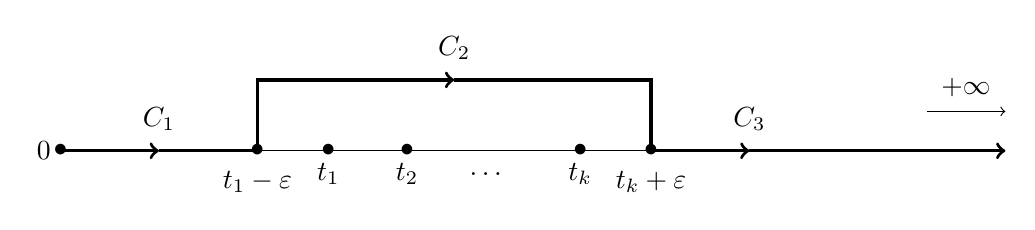
\begin{tikzpicture}
\draw (0,0) -- (12,0);
% primer trozo (C_1)
\draw[very thick,->] (0,0) -- (1.25,0);
\draw (1.25,0.4) node {$C_1$};
\draw[very thick] (1.25,0) -- (2.5,0);
% rect\'angulo (C_2):
\draw[very thick,->] (2.5,0) -- (2.5,0.9) -- (5,0.9);
\draw (5,1.3) node {$C_2$};
\draw[very thick] (5,0.9) -- (7.5,0.9) -- (7.5,0);
% tercer trozo (C_3):
\draw[very thick,->] (7.5,0) -- (8.75,0); 
\draw[very thick,->] (8.75,0) -- (12,0);
\draw (8.75,0.4) node {$C_3$};
% Points:
\draw (0,0) node {$\bullet$};
\draw (0,0) node[left] {$0$};
\draw (2.5,0) node {$\bullet$};
\draw (2.5,-0.4) node {$t_1-\eps$};
\draw (3.4,0) node {$\bullet$};
\draw (3.4,-0.3) node {$t_1$};
\draw (4.4,0) node {$\bullet$};
\draw (4.4,-0.3) node {$t_2$};
\draw (5.4,-0.3) node {$\dots$};
\draw (6.6,0) node {$\bullet$};
\draw (6.6,-0.3) node {$t_k$};
\draw (7.5,0) node {$\bullet$};
\draw (7.5,-0.4) node {$t_k+\eps$};
% +\infty:
\draw[->] (11,0.5) -- (12,0.5);
\draw (11.5,0.8) node {$+\infty$};
\end{tikzpicture}
\caption{An example of how the path $C$ ``avoids'' the singularities $t_1,t_2,\dots,t_k$ of $A(-t)$, from Theorem~\ref{teo:MAD-cont} (the radius of convergence of $A(t)$ must satisfy $R>t_1-\eps$).}
\label{fig:path-rectangle}
\end{figure}

\begin{proof}
The technique of the proof is somewhat similar to that in~\cite{NRV}, but more care must be taken to avoid the singularities.

Given $N \in \N \cup \{0\}$, the Mellin integral can be analytically continued to the half-plane $\Re(s) > -N-1$ as follows. For a fixed $\eps$ such that $t_1-R < \eps < \min\{\eta,R\}$ (note that necessarily $R \le t_1$ since $t_1$ is a singularity), separate the complete integral into three parts, each following the integration paths $C_1$, $C_2$ and $C_3$ (see Figure~\ref{fig:path-rectangle}; the upper corners of $C_2$ are $t_1-\eps+i\eps$ and $t_k+\eps+i\eps$, in order for $C_2$ to lie inside the $k$-punctured rectangle $T$ where $A(-t)$ is analytic). 
Next, further divide the integral along $C_1$ into two parts, so now we have four parts as follows:
\begin{equation}
\label{eq:parts}
\begin{aligned}
  H(s,x) &= \frac{1}{\Gamma(s)} \int_{t_k+\eps}^{\infty} A(-t) e^{-xt}t^{s-1}\,dt \\
  & \qquad + \frac{1}{\Gamma(s)} \int_{C_2} A(-t) e^{-xt}t^{s-1}\,dt 
\\
& \qquad + \frac{1}{\Gamma(s)} \int_0^{t_1-\eps} \left( A(-t) e^{-xt}
  - \sum_{n=0}^N P_{n}(x)\frac{(-t)^n}{n!} \right)t^{s-1}\,dt \\
  & \qquad + \frac{1}{\Gamma(s)} \int_0^{t_1-\eps} \sum_{n=0}^N P_{n}(x) 
  \frac{(-t)^n}{n!}t^{s-1} \,dt.
\end{aligned}
\end{equation}
In the first part, the integrand $e^{-xt}A(-t)t^{s-1}$ converges exponentially to $0$ when $t \to \infty$; it is dominated on arbitrary closed vertical strips of finite width, hence the integral is an entire function of $s$. Since $1/\Gamma(s)$ is entire, the complete first term is also.

In the second part, the integrand is again $e^{-xt}A(-t)t^{s-1}$ and since the path $C_2$ is finite and the integrand is analytic there, we again conclude that the integral is an entire function of~$s$. 

In the third part, note that the radius of convergence of $A(t)$ is $R>t_1-\eps$. The integrand is the product of $t^{s-1}$ with the tail of the generating series, $\sum_{n=N+1}^{\infty} P_{n}(x) (-t)^{n}/n!$, which is $\calO(t^{N+1})$ at $t=0$. Thus, for $\Re(s) > -N-1$, the complete integrand is $\calO(t^{N+\Re(s)})$ at $t=0$ (with the order constant depending only on~$x$) and hence is integrable on $[0,t_1-\eps]$ and dominated on closed vertical sub-strips of finite width of this section of the $s$-plane. Therefore the third integral is a holomorphic function of $s$ for $\Re(s) > -N-1$.

In the fourth part, we get
\begin{align}
\frac{1}{\Gamma(s)} \int_0^{t_1-\eps} \sum_{n=0}^N 
P_{n}(x) \frac{(-t)^n}{n!} t^{s-1} \,dt 
& = \frac{1}{\Gamma(s)} \sum_{n=0}^N P_{n}(x) \frac{(-1)^n}{n!}
\int_0^{t_1-\eps} t^{s+n-1} \,dt\nonumber \\ 
\label{eq:int-sum}
& = \frac{1}{\Gamma(s)}\sum_{n=0}^N P_{n}(x) 
\frac{(-1)^n}{n!} \frac{(t_1-\eps)^{s+n}}{s+n},
\end{align}
which is an entire function of $s$ because the simple pole of $\Gamma(s)$ at $s = -n$ cancels the simple zero of $s+n$ for $n=0,1,2,\dots$, leaving the non-zero residue $(-1)^n/n!$. 

Finally, if $s = -n$ with $0 \leq n \leq N$, the factor $1/\Gamma(s)$ in front of every integral is zero, so the first, second, and third parts in \eqref{eq:parts} vanish, while in the fourth part, the only non-zero summand in \eqref{eq:int-sum} corresponds to $n$, and yields the value $P_{n}(x)$ because of the residue of $\Gamma(s)$ at $-n = 0,1,2,\dots$, which is equal to $(-1)^n/n!$. Thus $H(-n,x) = P_{n}(x)$ for these $n$, and this completes the proof.
\end{proof}

In the next sections we show how to apply Theorem~\ref{teo:MAD-cont} to specific Appell sequences. In most cases, the singularities reduce to a single pole.
Before we proceed, we make some observations about the theorem.

\begin{figure}
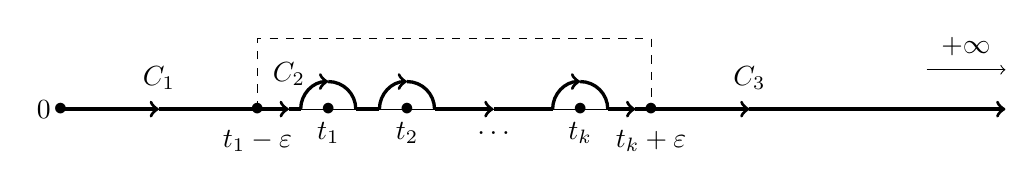
\begin{tikzpicture}
\draw (0,0) -- (12,0);
% primer trozo (C_1)
\draw[very thick,->] (0,0) -- (1.25,0);
\draw (1.25,0.4) node {$C_1$};
\draw[very thick] (1.25,0) -- (2.5,0);
%% rect\'angulo (C_2):
%\draw[very thick,->] (2.5,0) -- (2.5,1) -- (5,1);
%\draw (5,1.4) node {$C_2$};
%\draw[very thick] (5,1) -- (7.5,1) -- (7.5,0);
%% rect\'angulo:
\draw[dashed] (2.5,0) -- (2.5,0.9) -- (7.5,0.9) -- (7.5,0);
% tercer trozo (C_3):
\draw[very thick,->] (7.5,0) -- (8.75,0); % Esta flecha no estaba en el otro dibujo
\draw[very thick,->] (8.75,0) -- (12,0);
\draw (8.75,0.4) node {$C_3$};
% Points:
\draw (0,0) node {$\bullet$};
\draw (0,0) node[left] {$0$};
\draw (2.5,0) node {$\bullet$};
\draw (2.5,-0.4) node {$t_1-\eps$};
\draw (3.4,0) node {$\bullet$}; % Movido a la izquierda respecto al otro dibujo
\draw (3.4,-0.3) node {$t_1$};
\draw (4.4,0) node {$\bullet$}; % Movido a la derecha respecto al otro dibujo
\draw (4.4,-0.3) node {$t_2$};
\draw (5.5,-0.3) node {$\dots$};
\draw (6.6,0) node {$\bullet$}; % Movido a la derecha respecto al otro dibujo
\draw (6.6,-0.3) node {$t_k$}; 
\draw (7.5,0) node {$\bullet$}; 
\draw (7.5,-0.4) node {$t_k+\eps$};
% disks (radius=0.35) and C_2:
%% t_1 en (3.4,0): 
\draw[very thick] ({3.4+0.35},0) arc (0:90:0.35);
\draw[very thick,<-] ({3.4},0.35) arc (90:180:0.35);
\draw (2.9,0.45) node {$C_2$};
%% t_2 en (4.4,0):
\draw[very thick] ({4.4+0.35},0) arc (0:90:0.35);
\draw[very thick,<-] ({4.4},0.35) arc (90:180:0.35);
%% t_k en (6.6,0):
\draw[very thick] ({6.6+0.35},0) arc (0:90:0.35);
\draw[very thick,<-] ({6.6},0.35) arc (90:180:0.35);
%% segments in C_2
\draw[very thick,->] (2.5,0) -- (2.9,0);
\draw[very thick] (2.9,0) -- ({3.4-0.35},0);
\draw[very thick] ({3.4+0.35},0) -- ({4.4-0.35},0);
\draw[very thick,->] ({4.4+0.35},0) -- (5.5,0);
\draw[very thick] (5.5,0) -- ({6.6-0.35},0);
\draw[very thick,->] ({6.6+0.35},0) -- (7.3,0);
\draw[very thick] (7.3,0) -- (7.5,0);
% +\infty:
\draw[->] (11,0.5) -- (12,0.5);
\draw (11.5,0.8) node {$+\infty$};
\end{tikzpicture}
\caption{An alternative for the path $C_2$, as described in Remark~\ref{rem:disks}.}
\label{fig:path-disks}
\end{figure}

\begin{remark}
\label{rem:disks}
We have taken the $C_2$ part of the path $C$ as the upper part of a rectangle. This is not essential since for functions which are analytic in a simply connected domain, the integral is independent of the path. For instance, we could also take the $C_2$ part as in Figure~\ref{fig:path-disks} (again with $R>t_1-\eps$). The most common (and easy) case of the previous theorem is when $A(-t)$ has only one singularity, which we call~$t_0$. In this case, we usually describe the $C_2$ part of the path as a semicircle of radius $\eps$ centered on $t_0$, as in Figure~\ref{fig:path-disk}. In many cases, the radius of convergence of $A(-t)$ is $R=t_0$, and then we can take any $\eps>0$.
\end{remark}

\begin{figure}
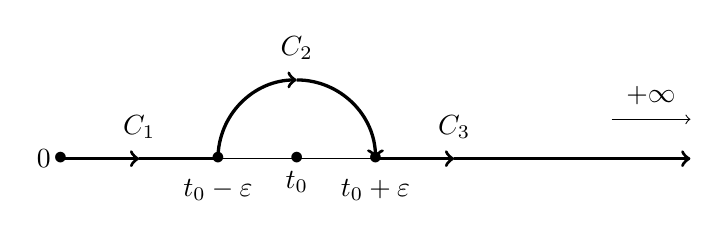
\begin{tikzpicture}
%real negatives line
\draw (-3,0) -- (5,0);
%inner circle and connection with outer circle
\draw[very thick,<-] (1,0) arc (0:90:1);
\draw[very thick,<-] (0,1) arc (90:180:1);
\draw (0,-0.3) node {$t_0$};
\draw (-3,0) node[left] {$0$};
\draw (0,0) node {$\bullet$};
\draw (-3,0) node {$\bullet$};
\draw (-1,0) node {$\bullet$};
\draw (1,0) node {$\bullet$};
\draw (4.5,0.8) node {$+\infty$};
\draw[very thick,->] (-3,0) -- (-2,0);
\draw[very thick] (-2,0) -- (-1,0);
\draw[very thick,->] (1,0) -- (2.0,0);
\draw[very thick,->] (2.0,0) -- (5,0);
\draw[->] (4,0.5) -- (5,0.5);
%\draw[very thick] (0.7,0) arc (360:195:0.7) -- (-3,0);
%arrows
%\draw[thick, <-] (1,0) arc(0:45:1);
%\draw[thick, ->] (1.5,0.4) -- (3,0.4);
%\draw[thick, ->] (-2.5,0.4) -- (-1.5,0.4);
%nodes
\draw (0,1.4) node {$C_2$};
\draw (-1,-0.4) node {$t_0-\eps$};
\draw (1,-0.4) node {$t_0+\eps$};
\draw (2.0,0.4) node {$C_3$};
\draw (-2.0,0.4) node {$C_1$};
\end{tikzpicture}
\caption{An example of how the path $C$ that ``avoids'' a unique singularity $t_0$ of $A(-t)$.}
\label{fig:path-disk}
\end{figure}

\begin{remark}
\label{rem:above-under}
For simplicity, assume that we have a unique singularity at $t_0$, as described in the previous remark, with the path $C$ passing above the singularity as shown in Figure~\ref{fig:path-disk}, and~$C_2$ equal to a semicircle. Clearly, we could also take the path $C$ passing under the singularity~$t_0$, obtaining two different functions $H(s,x)$ satisfying $H(-n,x)=P_n(x)$. Let $C^{+}$ denote the path going over $t_0$ (as in the figure) and $C^{-}$ the path going under $t_0$, and let us denote by $H^{+}(s,x)$ and $H^{-}(s,x)$ the corresponding functions $H(s,x)$. Then, by Cauchy's residue theorem,
\begin{align*}
  H^-(s,x) &= \frac{1}{\Gamma(s)} \int_{C^-} A(-t)e^{-xt} t^{s-1}\,dt \\
  &= \frac{1}{\Gamma(s)} \int_{C^+} A(-t)e^{-xt} t^{s-1}\,dt 
  + \frac{1}{\Gamma(s)} \int_{|t-t_0|=\eps} A(-t)e^{-xt} t^{s-1}\,dt \\
  &= H^+(s,x) + \frac{2\pi i}{\Gamma(s)} \Res(A(-t)e^{-xt} t^{s-1},t=t_0)
\end{align*}
in the right plane $\Re(s) > 0$. By analytic continuation, this relation between $H^-(s,x)$ and $H^+(s,x)$ is also true in the complex $s$-plane. 
If $A(-t)$ has a pole of order $1$ at $t_0$, let us write $A(-t) = \sum_{k=-1}^\infty a_{k} (t-t_0)^k$; 
then, it is easy to see that $\Res(A(-t)e^{-xt} t^{s-1},t=t_0) = a_{-1} e^{-t_0 x}t_0^{s-1}$.
%% ESO LO CALCULA Mathematica CON
%% Series[(t - t0)^{-1}*Exp[-x*t]*t^(s-1), {t, t0, 2}]

In the case of more that one singularity, as in Figure~\ref{fig:path-disks}, we can also conceive of paths that zigzag between singularities, some going over and some under (for instance, with semicircles above and below the horizontal axis). This will generate many different functions $H(s,t)$ but, again, they will be related by the residues at the singularities.
\end{remark}

\begin{remark}
For certain generating functions $A(t)$ such that $A(-t)$ has a pole at a certain $t_0>0$, Theorem~\ref{teo:MAD-cont} might be superfluous. For instance, let us assume given $A(t)$ and the corresponding Appell polynomials $P_n(x)$, and let $\widetilde{A}(t) = A(-t)$, with corresponding Appell polynomials $\widetilde{P}_n(x)$; if $A(-t)$ has a pole at $t_0>0$, it becomes $-t_0$ (negative) for $\widetilde{A}(-t)$, and perhaps $\widetilde{A}(t)$ satisfies the hypotheses of \cite[Theorem~1]{NRV}. 
With this notation, 
\[
\sum_{n=0}^\infty P_{n}(x)\frac{t^n}{n!} = A(t) e^{xt} 
= \widetilde{A}(-t) e^{(-x)(-t)} 
= \sum_{n=0}^\infty \widetilde{P}_{n}(-x) \frac{(-t)^n}{n!},
\]
so $P_{n}(x) = (-1)^n \widetilde{P}_{n}(-x)$. Consequently, if $\widetilde{H}(s,x)$ is the $s$-entire function that satisfies $\widetilde{H}(-n,x) = \widetilde{P}_n(x)$, the new $s$-entire function $H(s,x) = e^{i\pi s} \widetilde{H}(s,-x)$ (or $e^{-i\pi s} \widetilde{H}(s,-x)$) satisfies
\[
  H(-n,x) = e^{-i\pi n} \widetilde{H}(-n,-x) = (-1)^n \widetilde{P}_{n}(-x) = P_{n}(x).
\]
In any case, the trick above mention cannot be used if, for instance, $A(-t)$ has poles both at $t_0$ and at $-t_0$. In particular, this happens for $A(t) = 1/(1-t^2)$.
\end{remark}

\begin{remark}
Sometimes, a clever use of Theorem~\ref{teo:MAD-cont} allows us to find in a simple way the function $H(s,x)$ corresponding to \eqref{E:Appell_GF} if $A(-t)$ has more that one pole on $(0,\infty)$. To exemplify it, let us assume that we have $t_1$ and $t_2$ satisfying $0<t_1<t_2$ and
\[
  A(t) = \frac{\widetilde{A}(t)}{(t+t_1)(t+t_2)},
\]
for a function $\widetilde{A}(t)$ without singularities. 
Let us take the partial fraction decomposition
\[
\frac{1}{(t+t_1)(t+t_2)} = \frac{k_1}{t+t_1} + \frac{k_2}{t+t_2},
\qquad k_1=(t_2-t_1)^{-1}, \quad k_2=(t_1-t_2)^{-1},
\]
as well as the Appell sequences
\[
  \frac{\widetilde{A}(t)}{t+t_j}e^{xt} = \sum_{n=0}^{\infty} P_n^j(x)\frac{t^n}{n!},
  \qquad j=1,2.
\]
Then,
\begin{equation*}
  \sum_{n=0}^{\infty} P_n(x)\frac{t^n}{n!} = A(t) e^{xt}
  = k_1 \frac{\widetilde{A}(t)}{t+t_1}e^{xt} 
  + k_2\frac{\widetilde{A}(t)}{t+t_2}e^{xt} \\
  = k_1 \sum_{n=0}^{\infty} P^{1}_n(x)\frac{t^n}{n!} 
  + k_2 \sum_{n=0}^{\infty} P^{2}_n(x)\frac{t^n}{n!},
\end{equation*}
%\begin{align*}
%  \sum_{n=0}^{\infty} P_n(x)\frac{t^n}{n!} &= A(t) e^{xt}
%  = k_1 \frac{\widetilde{A}(t)}{t+t_1}e^{xt} 
%  + k_2\frac{\widetilde{A}(t)}{t+t_2}e^{xt} \\
%  &= k_1 \sum_{n=0}^{\infty} P^{1}_n(x)\frac{t^n}{n!} 
%  + k_2 \sum_{n=0}^{\infty} P^{2}_n(x)\frac{t^n}{n!},
%\end{align*}
so $P_n(x) = k_1 P^{1}_n(x) + k_2 P^{2}_n(x)$.

It is clear that the radius of convergence of $\frac{\tilde{A}(t)}{t+t_j}$ is $t_j$, for $j=1,2$, and we can apply Theorem~\ref{teo:MAD-cont} in both cases, obtaining  $s$-entire functions $H_j(s,x)$ such that $H_j(-n,x) = P^{j}_n(x)$. Consequently, taking
\[
H(s,x) = k_1 H_1(s,x) + k_2 H_2(s,x)
\]
we have $H(-n,x) = P_n(x)$, as desired.
\end{remark}

%-----------
\section{The case $A(t) = 1/(1-t)^r$}
\label{sec:1-tr}
%-----------

For completeness, and to compare it with the case $A(t) = 1/(1+t)^r$ that will be explored in the next section, we begin with an example that does not require the extension given in Theorem~\ref{teo:MAD-cont} of this paper because $A(-t) = 1/(1+t)^r$ does not have singularities on $[0,\infty)$. However, perhaps the most interesting case, which corresponds to $r=1$, was not studied in~\cite{NRV}. 

Let $\{P_n^{(r-)}(x)\}_{n=0}^{\infty}$ be the polynomials defined by
\begin{equation}
\label{eq:pol.1-t}
  \frac{1}{(1-t)^r} e^{xt} = \sum_{n=0}^{\infty} P_n^{(r-)}(x) \frac{t^n}{n!},
  \qquad |t| < 1.
\end{equation}

The case $r=1$ is of interest on its own. In this particular case, for $|t|<1$ we have
\[
  \frac{1}{1-t} e^{xt} 
  = \Biggl(\sum_{j=0}^{\infty} t^j \Biggr) \Biggl(\sum_{j=0}^{\infty} \frac{(xt)^j}{j!} \Biggr) 
  = \sum_{n=0}^{\infty} \frac{t^n}{n!} \Biggl(\sum_{k=0}^{n} \frac{x^{n-k}}{(n-k)!}k! \Biggr)
\]
and hence, equating coefficients in \eqref{eq:pol.1-t}, we get
\begin{equation}
\label{eq:pol.en}
  P_n^{(1-)}(x) = n!\,\Big(1+x+\frac{x}{2}+ \cdots +\frac{x^n}{n!}\Big) = n!\,e_n(x). 
\end{equation}
The $e_n(x)$ are called the truncated exponential polynomials.

For general $r$, we have
\begin{equation*}
  H^{(r-)}(s,x) = \frac{1}{\Gamma(s)} \int_{0}^{\infty} e^{-xt}(1+t)^{-r} t^{s-1} \,dt,
  \quad \Re(s)>0,\ \Re(x)>0,
\end{equation*}
and \cite[Theorem~1]{NRV} (and also Theorem~\ref{teo:MAD-cont} of this paper, of course) implies that this function can be analytically continued to a $s$-entire function satisfying $H^{(r-)}(-n,x) = P_n^{(r-)}(x)$. Actually, $H^{(r-)}(s,x)$ is an old well-known function in the mathematical literature, as we now show.

Let us recall that Tricomi's confluent hypergeometric function is 
\[
  \Psi(a,c;x) =
  \frac{\Gamma(1-c)}{\Gamma(a+1-c)} \,{}_1 F_1(a, c; t)
  + \frac{\Gamma(b-1)}{\Gamma(a)} t^{1-c} \,{}_1F_1(a+1-c, 2-c; t)
\]
(it is also denoted by $U(a,c,x)$, see \cite[\S\,6.5, equation~(2)]{EMOT-HTF-v1} or \cite[p.~242 in \S\,5.5.2]{MOT}).
This function, that will appear several other times in this paper, is often defined as the Mellin transform
\begin{equation*}
  \Psi(a,c;x) = \frac{1}{\Gamma(a)} \int_0^{\infty}e^{-xt}(1+t)^{c-a-1} t^{a-1}\,dt, 
  \quad \Re(a)>0,\ \Re(x)>0,
\end{equation*}
and then extended by analytic continuation.

With our notation, $H^{(r-)}(s,x) = \Psi(s,s-r+1;x)$ and $H^{(r-)}(-n,x) = P_n^{(r-)}(x)$.
But, when $s=-n$, by \cite[\S\,6.9.2, equation~(36)]{EMOT-HTF-v1} we have
\begin{equation*}
  \Psi(-n,-n-r+1;x) = (-1)^n n!\,L_{n}^{(-n-r)}(x),
\end{equation*}
where
\[
  L_{n}^{(\alpha)}(x) = \sum_{k=0}^{n} \binom{n+\alpha}{n-k} \frac{(-x)^k}{k!}
\]
denotes the (generalized) Laguerre polynomial of degree $n$ and order~$\alpha$ (here, $\binom{n+\alpha}{n-k}$ is the generalized binomial coefficient). Consequently, $P_n^{(r-)}(x) = (-1)^n n!\,L_{n}^{(-n-r)}(x)$.

The case $r=1$ yields
\begin{equation*}
  H^{(1-)}(s,x) = \frac{1}{\Gamma(s)} \int_{0}^{\infty} e^{-xt}(1+t)^{-1} t^{s-1} \,dt 
  = \Psi(s,s;x),
\end{equation*}
and the function $H^{(1-)}(s,x)$ analytically continued to the $s$-plane satisfies $H(-n,x) = n!\,e_n(x)$.

Now, note that one of the properties of the incomplete Gamma function
\begin{equation}
\label{eq:incompletes}
  \Gamma(s,x) = \int_x^{\infty} e^{-t} t^{s-1} \,dt,
\end{equation}
is the following relation (see, for instance, \cite[\S\,9.1, equation~(4)]{EMOT-HTF-v2}):
\begin{equation}
\label{eq:gamm-conf}
  \Gamma(s,x) = e^{-x}\Psi(1-s,1-s;x).
\end{equation}
Hence, 
\begin{equation}
\label{eq:H-case1-t}
  H^{(1-)}(s,x) = e^x \Gamma(1-s,x),
\end{equation}
and consequently
\begin{equation}
\label{eq:H1-n}
  H^{(1-)}(-n,x) = e^x \Gamma(n+1,x) = n! \,e_{n}(x).
\end{equation}
Thus we recover a nice property of the incomplete Gamma function (see, for instance, \cite[8.4.8]{Par-NIST}):
\begin{equation}
\label{eq:incompleten}
  \Gamma(n,x) = (n-1)!\,e^{-x} e_{n-1}(x), \quad n\in\N.
\end{equation}

%-----------
\subsection{McBride polynomials}
%-----------
Let us finish this section by mentioning some polynomials related to what has been shown and that have been studied in the mathematical literature.
They are the McBride polynomials $\{e_n^{\lambda}(x)\}_{n=0}^{\infty}$, defined by (see, for instance, \cite[equation~(12)]{DCS})
\[
  \sum_{n=0}^{\infty} t^n e_n^{\lambda}(x) = e^{xt} \, \frac{\Gamma{(\lambda+1})}{(1-t)^{\lambda}}.
\]
These polynomials are an easy variation of $\{P_n^{(\lambda-)}(x)\}_{n=0}^{\infty}$, and thus we have that 
$\Psi(s,s-\lambda+1;x)$ satisfies
\[
  \Psi(-n,-n-\lambda+1;x) = n!\,\Gamma(\lambda+1)e_n^{\lambda}(x).
\]

%-----------
\section{The case $A(t) = 1/(1+t)^r$}
\label{sec:1+tr}
%-----------

Let $\{P_n^{(r+)}(x)\}_{n=0}^{\infty}$ be the polynomials defined by
\begin{equation*}
\frac{1}{(1+t)^r} e^{xt} = \sum_{n=0}^{\infty} P_n^{(r+)}(x) \frac{t^n}{n!},
\qquad |t| < 1.
\end{equation*}

Note that in this case the integral
\begin{equation*}
H^{(r+)}(s,x) = \frac{1}{\Gamma(s)}\int_{0}^{\infty} e^{-xt}(1-t)^{-r} t^{s-1} \,dt
\end{equation*}
does not converge because $A(-t) = (1-t)^{-r}$ has a pole at $t_0=1$. 
However, we can apply Theorem~\ref{teo:MAD-cont}, and thus we can consider
\begin{equation*}
H^{(r+)}(s,x) = \frac{1}{\Gamma(s)}\int_{C} e^{-xt}(1-t)^{-1} t^{s-1} \,dt,
\end{equation*}
where the path $C$ goes from $0$ to $\infty$ but jumps over the pole $t_0=1$ (as shown in Figure~\ref{fig:path-disk}), and Theorem~\ref{teo:MAD-cont} guarantees that $H^{(r+)}(s,x)$ can be analytically continued to an $s$-entire function that satisfies $H^{(r+)}(-n,x) = P_n^{(r+)}(x)$. 

To identify the function $H^{(r+)}(s,x)$, let us start by noticing that for $H^{(r-)}(s,x)$ we had, for $\Re(s) > 0$ and $\Re(x) > 0$,
\begin{equation*}
  H^{(r-)}(s,x) = \Psi(s,s-r+1;x) = \frac{1}{\Gamma(s)} \int_0^{\infty }e^{-xt}(1+t)^{-r} t^{s-1}\,dt.
\end{equation*}

\begin{figure}
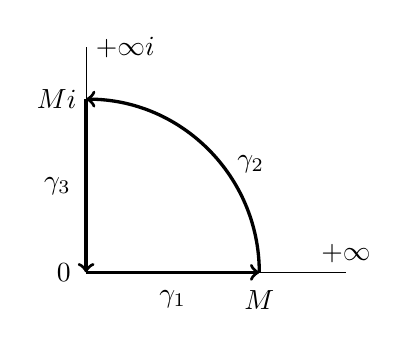
\begin{tikzpicture}[scale=0.55]
\draw (-3,0) -- (3,0) node[above] {$+\infty$};
\draw (-3,0) -- (-3,5.2) node[right] {$+\infty i$};
\draw[very thick,->] (-3,0) -- (1,0);
\draw[very thick,->] (1,0) arc (0:90:4);
\draw[very thick,->] (-3,4) -- (-3,0);
\draw (-3,0) node[left=2] {$0$};
\draw (0.8,2.5) node {$\gamma_2$};
\draw (-3,2) node[left=2] {$\gamma_3$};
\draw (-1,0) node[below=3] {$\gamma_1$};
\draw (1,0) node[below=3] {$M$};
\draw (-3,4) node[left] {$Mi$};
\end{tikzpicture}
\caption{Path for transforming an integral on $(0,+\infty)$ into an integral on $(0,+\infty i)$.}
\label{fig:path-analytic-cont}
\end{figure}

If we change the path of integration of $H^{(r-)}(s,x)$ to the positive imaginary axis, we have that
\begin{equation}
\label{eq:analytic-cont}
  \frac{1}{\Gamma(s)}\int_0^{\infty i}e^{-xt}(1+t)^{-r} t^{s-1}\,dt
\end{equation}
is convergent for $\Re(s)>0$ and $-\pi < \arg(x) <0$. Let $f(t) = e^{-xt}(1+t)^{-r} t^{s-1}$ and consider the integral $\int_{\gamma} f(t)\,dt$, where $\gamma$ is the composition of the paths $\gamma_1, \gamma_2$ and $\gamma_3$ given in Figure~\ref{fig:path-analytic-cont}. Since $f(t)$ has no singularities inside the contour $\gamma$, $\int_{\gamma} f(t)\,dt = \int_{\gamma_1} f(t)\,dt + \int_{\gamma_2} f(t)\,dt + \int_{\gamma_3} f(t)\,dt = 0$, and it is easy to prove that $\int_{\gamma_2} f(t)\,dt = 0$ when $M\to \infty$ (because of the term $e^{-xt}$ in the integrand).
Hence $\int_0^{\infty} f(t)\,dt = \int_{0}^{\infty i} f(t)\,dt$, so $H^{(r-)}(s,x)$ is equal to \eqref{eq:analytic-cont} in the overlapping domain $-\pi/2 < \arg(x) <0$. By the same reasoning, we can change the path to the negative real axis $t\in [0,-\infty)$, and thus
\begin{equation}
\label{eq:H1-aux}
  H^{(r-)}(s,x) = \frac{1}{\Gamma(s)} \int_0^{-\infty}e^{-xt}(1+t)^{-r} t^{s-1}\,dt,
\end{equation} 
where the path passes above the pole at $t_0=-1$, similarly to  Figure~\ref{fig:path-disk}, but on the negative real axis.

Finally, substituting $z=-t=e^{i\pi}t$ in \eqref{eq:H1-aux}, we get
\begin{equation*}
  H^{(r-)}(s,xe^{i\pi}) = \Psi(s,s-r+1;xe^{i\pi}) 
  = \frac{e^{i\pi s}}{\Gamma(s)} \int_C e^{-xz}(1-z)^{-r} z^{s-1}\,dz,
\end{equation*}
with $C$ as in Figure~\ref{fig:path-disk} (with $z_0=1$).
Then,
\begin{equation}
\label{eq:Hr-1+t}
  H^{(r+)}(s,x) = \frac{1}{\Gamma(s)} \int_{C} e^{-xz}(1-z)^{-r} z^{s-1}\, dz 
  %= e^{-\pi i (s-1)}\Psi(s,s-r+1;xe^{\pi i})
  = e^{-\pi i s}\Psi(s,s-r+1;xe^{\pi i})
\end{equation}
is a function that satisfies $H^{(r+)}(-n,x) = P_n^{(r+)}(x)$.

Note that if we substitute $z = te^{-i\pi}$ instead of $z = te^{i\pi}$ we obtain a different special function $H^{(r+)}(s,x)$ which satisfies $H^{(r+)}(-n,x) = P_n^{(r+)}(x)$ (see, for instance,~\cite{Temme})
\[
  \widetilde{H}^{(r+)}(s,x) = e^{\pi i s}\Psi(s,s-r+1;e^{-i\pi}x).
\]
In this case $C$ passes under the pole $t_0=1$, which is related to Remark~\ref{rem:above-under}. We will use this reasoning for obtaining $H^{(r+)}(s,x)$ and $\widetilde{H}^{(r+)}(s,x)$ many other times in this paper, but we will omit the details from now on.

The case $r=1$ is interesting for its own sake. We get
\begin{equation}
\label{eq:pol.1+t}
  \frac{1}{1+t} e^{xt} = \sum_{n=0}^{\infty} P_n^{(1+)}(x) \frac{t^n}{n!},
  \qquad |t| < 1,
\end{equation}
and it is easy to prove that $P_n^{(1+)}(x) = (-1)^n n!\, e_n(-x)$. Of course, this can be easily deduced from \eqref{eq:pol.1-t} and \eqref{eq:pol.en} changing $x$ to $-x$ and $t$ to~$-t$.

A direct consequence of \eqref{eq:Hr-1+t} together with \eqref{eq:gamm-conf} is
\begin{equation*}
  \Gamma(-s+1,xe^{\pm\pi i}) = e^xe^{\pm\pi i s} \frac{1}{\Gamma(s)} 
  \int_{C} \frac{e^{-xt}}{1-t} t^{s-1}\, dt 
\end{equation*}
and
\begin{equation}
\label{eq:H-case1+t}
  H^{(1+)}(s,x) 
  % = \frac{1}{\Gamma(s)} \int_{C} \frac{e^{-xt}}{1-t} t^{s-1} \,dt 
  = \Gamma(-s+1,xe^{\pm \pi i}) e^{-x}e^{\mp \pi i s}.
\end{equation}

%-----------
\subsection{Appell-type Changhee polynomials}
%-----------

As in Section~\ref{sec:1-tr}, let us finish this section by mentioning another family of Appell polynomials with a proper name. The so-called Appell-type Changhee polynomials, $\{\Ch_n^*(x)\}_{n=0}^{\infty}$, introduced in~\cite{LJSCK}, are defined by
\begin{equation*}
  \frac{2}{2+t}e^{xt} = \sum_{n=0}^{\infty} \Ch_n^{*}(x) \frac{t^n}{n!},
  \qquad |t| < 2.
\end{equation*}
The generating function $\frac{2}{2+t}e^{xt}$ is closely related to $\frac{1}{1+t}e^{xt}$ by means of the change of variables $t \mapsto 2t$ and $x \mapsto x/2$. It is easy to check that the  Appell-type Changhee polynomials are related to the truncated exponential polynomials by the equation
\begin{equation*}
  \Ch_n^{*}(x) = \frac{(-1)^n n!}{2^n}e_n(-2x).
\end{equation*}
To find the special function that satisfies $H(-n,x) = \Ch_n^*(x)$ for $n=0,1,2,\dots$, let us take the integral
\begin{equation*}
  H(s,x) = \frac{2}{\Gamma(s)}\int_{C} \frac{e^{-xt}}{2-t}t^{s-1}\,dt,
\end{equation*}
where now $C$ is a path avoiding the pole at $t_0=2$. By changing $t \mapsto 2t$ in the integral and recalling~\eqref{eq:H-case1+t}, we get
\begin{equation*}
  H(s,x) = 2^{s} \Gamma(-s+1,2xe^{\pm \pi i})e^{-2x}e^{\mp \pi i s}.
\end{equation*}

%-----------
\section{The cases $A(t) = 1/(1-t^k)$ and $A(t) = 1/(1+t^k)$}
\label{sec:1+-tk}
%-----------

In this section we are going to study together the two cases $A(t) = 1/(1-t^k)$ and $A(t) = 1/(1+t^k)$, whose corresponding Appell polynomials will be denoted by $P_n^{[k]}(x)$ and $Q_n^{[k]}(x)$. We study these cases simultaneously because we will obtain two special functions $H_{j}^{[k]}(s,x)$ such that $H_{j}^{[k]}(-n,x)$ (both for $j=1,2$) is equal to $P_n^{[k]}(x)$ or $Q_n^{[k]}(x)$ depending on $k$ being even or odd.

First, let us denote by $\{P_n^{[k]}(x)\}_{n=0}^{\infty}$ the polynomials defined by
\begin{equation*}
  \frac{1}{1-t^k} e^{xt} = \sum_{n=0}^{\infty} P_n^{[k]}(x) \frac{t^n}{n!},
  \qquad |t| < 1.
\end{equation*}

Of course, the case $k=1$ gives us $P_n^{(1)}(x) = n!\,e_n(x)$, and they are given by
\[
P_n^{[k]}(x) = n!\sum_{j=0}^{\lfloor {n}/{k} \rfloor} \frac{x^{n-kj}}{(n-kj)!}
\]
(these polynomials are studied, for instance, in \cite[(1.19)]{KYA}, where they are denoted by ${}_{[k]}e_n(x)$).

In this case, we get that
\begin{equation*}
  H^{[k]}(s,x) = \frac{1}{\Gamma(s)}\int_{0}^{\infty} \frac{e^{-xt}}{1-(-t)^k} t^{s-1}\,dt 
= 
\begin{cases}
  \frac{1}{\Gamma(s)}\int_{0}^{\infty} e^{-xt}(1-t^k)^{-1} t^{s-1}\,dt, 
    & \text{ if } k \text{ even,} \\[6pt]
  \frac{1}{\Gamma(s)}\int_{0}^{\infty} e^{-xt}(1+t^k)^{-1} t^{s-1}\,dt, 
    & \text{ if } k \text{ odd.} 
\end{cases}
\end{equation*}
%\begin{align*}
%  H^{[k]}(s,x) &= \frac{1}{\Gamma(s)}\int_{0}^{\infty} \frac{e^{-xt}}{1-(-t)^k} t^{s-1}\,dt \\
%&= 
%\begin{cases}
%  \frac{1}{\Gamma(s)}\int_{0}^{\infty} e^{-xt}(1-t^k)^{-1} t^{s-1}\,dt, 
%    & \text{ if } k \text{ even,} \\[6pt]
%  \frac{1}{\Gamma(s)}\int_{0}^{\infty} e^{-xt}(1+t^k)^{-1} t^{s-1}\,dt, 
%    & \text{ if } k \text{ odd.} 
%\end{cases}
%\end{align*}

On the other hand, if $\{Q_n^{[k]}(x)\}_{n=0}^{\infty}$ are the polynomials defined by
\begin{equation*}
  \frac{1}{1+t^k} e^{xt} = \sum_{n=0}^{\infty} Q_n^{[k]}(x) \frac{t^n}{n!},
  \qquad |t| < 1,
\end{equation*}
where
\[
  Q_n^{[k]}(x) = n!\sum_{j=0}^{\lfloor {n}/{k} \rfloor} \frac{(-1)^j x^{n-kj}}{(n-kj)!},
\]
we get that
\begin{equation*}
  H^{[k]}(s,x) 
  = \frac{1}{\Gamma(s)}\int_{0}^{\infty} \frac{e^{-xt}}{1+(-t)^k} t^{s-1}\,dt 
  = 
\begin{cases}
  \frac{1}{\Gamma(s)}\int_{0}^{\infty} e^{-xt}(1+t^k)^{-1} t^{s-1}\, dt, 
    & \text{ if } k \text{ even,} \\[6pt]
  \frac{1}{\Gamma(s)}\int_{0}^{\infty} e^{-xt}(1-t^k)^{-1} t^{s-1}\, dt, 
    & \text{ if } k \text{ odd.} 
\end{cases}
\end{equation*}
%\begin{align*}
%  H^{[k]}(s,x) 
%  &= \frac{1}{\Gamma(s)}\int_{0}^{\infty} \frac{e^{-xt}}{1+(-t)^k} t^{s-1}\,dt \\
%  &= 
%\begin{cases}
%  \frac{1}{\Gamma(s)}\int_{0}^{\infty} e^{-xt}(1+t^k)^{-1} t^{s-1}\, dt, 
%    & \text{ if } k \text{ even,} \\[6pt]
%  \frac{1}{\Gamma(s)}\int_{0}^{\infty} e^{-xt}(1-t^k)^{-1} t^{s-1}\, dt, 
%    & \text{ if } k \text{ odd.} 
%\end{cases}
%\end{align*}

Then we could argue that, for $k=1,2,3,\dots$, the function
\begin{equation*}
  H_1^{[k]}(s,x) = \frac{1}{\Gamma(s)}\int_{0}^{\infty} e^{-xt}(1+t^k)^{-1} t^{s-1}\, dt
\end{equation*}
can be analytically continued to the $s$-complex plane (in this case \cite[Theorem~1]{NRV} is enough to do it) and satisfies $H_1^{[k]}(-n,x) = P_n^{[k]}(x)$ if $k$ is odd and $H_1^{[k]}(-n,x) = Q_n^{[k]}(x)$ if $k$ is even.

On the other hand, we notice that the integral
\[
  \int_{0}^{\infty} e^{-xt}(1-t^k)^{-1} t^{s-1}\, dt
\]
does not converge for any $k=1,2,3,\dots$. However, we can consider instead
\begin{equation*}
  H_2^{[k]}(s,x) = \frac{1}{\Gamma(s)}\int_{C} e^{-xt}(1-t^k)^{-1} t^{s-1}\, dt,
\end{equation*}
which can be analytically continued to the $s$-complex plane as described in Theorem~\ref{teo:MAD-cont}.
Then, $H_2^{[k]}(-n,x) = Q_n^{[k]}(x)$ if $k$ is odd and $H_2^{[k]}(-n,x) = P_n^{[k]}(x)$ if $k$ is even.

Next, we show how to express $H_1^{[k]}(s,x)$ and $H_2^{[k]}(s,x)$ in terms of previously known special functions. Both of them are particular cases of Meijer $G$-functions, a remarkable family of functions of one variable, each of them determined by finitely many indices. By definition, via the Mellin-Barnes integral representation, the Meijer $G$-function is
\[
  G_{p,q}^{m,n}\parenG{a_1, \dots, a_p}{b_1, \dots, b_q}{z} \\ 
  = \frac{1}{2\pi i} \int_L \frac{\prod_{j=1}^m\Gamma(b_j-t) 
  \prod_{j=1}^n \Gamma(1-a_j+t)}{\prod_{j=m+1}^q \Gamma(1-b_j+t) \prod_{j=n+1}^p \Gamma(a_j-t)}z^t\, dt
\]
where the integration path $L$ separates the poles of the factors $\Gamma(b_j-t)$ 
from those of the factors $\Gamma(1-a_j+t)$, with three possible choices for this path 
(for details, see \cite[\S\,16.17]{AsOl-NIST} or \cite{BS} and the references therein). 

Meijer $G$-functions have proved useful for generalizing a huge class of functions, including elementary functions, gamma functions, Bessel functions, hypergeometric functions, and so on. If $A(t)$ can be written as a Meijer $G$-function as 
$A(-t) = G_{p,q}^{m,n}\tparenG{a_1, \dots, a_p}{b_1, \dots, b_q}{\eta t}$ 
for some constant~$\eta$, then
\begin{equation}
\label{eq:MG}
  \int_{0}^{\infty} G_{p,q}^{m,n}\parenG{a_1, \dots, a_p}{b_1, \dots, b_q}{\eta t}e^{-xt}t^{s-1}\,dt 
  = x^{-s}G_{p+1,q}^{m,n+1}\parenG{1-s,a_1, \dots, a_p}{b_1, \dots, b_q}{\frac{\eta}{x}}
\end{equation}
(see \cite[\S\,5.5.2]{EMOT-HTF-v1}). 
However, in our case we have  
$1/(1+t^k) = G_{1,1}^{1,1}\tparenG{0}{0}{t^k}$, 
which is not of this form. Hence, the identity \eqref{eq:MG} alone isn't enough to compute the integral \eqref{E:Mellin_GF_def}, and for this reason we need some auxiliary results involving Mellin transforms.

%% EN \cite[p.~870]{BS} PONE, APROXIMADAMENTE, ``for a certain path $L$''.
%% EN \cite[\S\,16.17]{AsOl-NIST} PONE ``where the integration path $L$ separates 
%% the poles of the factors $\Gamma(b_j-t)$ from those of the factors $\Gamma(1-a_j+t)$, 
%% with three possible choices for this path''.
%% HAY TRES POSIBILIDADES PARA EL PATH $L$ DEPENDIENDO DE LOS PAR\'AMETROS.

\begin{theorem}
\label{teo:int1+tk}
For $k\in \mathbb{N}$ we have that
\begin{equation*}
  \frac{1}{\Gamma(s)} \int_{0}^{\infty} \frac{e^{-xt}}{1+t^k} t^{s-1} \,dt 
  = \frac{(2\pi)^{\frac{1-k}{2}}}{\sqrt{k}\,\Gamma(s)}\, G_{k+1,1}^{1,k+1}
  \parenG{1,\frac{k-1}{k},\dots, \frac{1}{k}, \frac{s}{k}}{s/k}{\left(\frac{k}{x}\right)^k}, 
\end{equation*}
where the function $G_{k+1,1}^{1,k+1}$ is a Meijer $G$-function. 
\end{theorem}

We need the following lemmas to prove the above theorem. 
We refer Lemma~\ref{lem:mellin-tran} to \cite[Chapter VI]{EMOT-TIT-v1}, and Lemma~\ref{lem:parseval} to~\cite[\S\,8.2 and \S\,8.3]{DB} or \cite[Theorem~73, p.~95]{Tit}.

\begin{lemma}
\label{lem:mellin-tran}
Let $\mathcal{M}\{f(t)\}(s)$ denote the Mellin transform of a suitable function $f(t)$. Then
\[
  \mathcal{M}\{e^{-xt}\}(s) = \Gamma(s)x^{-s}, \quad 0<\Re(s),
\]
and
\[
  \mathcal{M}\left\{\frac{1}{1+t^k}\right\}(s) 
  = \frac{\pi}{k} \csc\Big( \frac{\pi}{k}s \Big) 
  = \frac{1}{k} \Gamma \Big(\frac{s}{k}\Big) \Gamma\Big(1-\frac{s}{k}\Big), \quad 0<\Re(s)<k.
\]
\end{lemma}


\begin{lemma}[Parseval's formula for Mellin transforms]
\label{lem:parseval}
Let $f_1(t)$, $f_2(t)$ be two functions with Mellin transforms $\tilde{f}_{j}(t) = \mathcal{M}\{f_{j}(t)\}(s)$, $j = 1,2$, in the strips $\alpha_{1,2} < \Re(s) < \beta_{1,2}$, respectively. Take $c \in \mathbb{R}$ such that $\alpha_1< c <\beta_1$ and suppose that $f_1(t)t^c$ and $f_2(t)t^{\Re(s) -c}$ belong to $L^2((0,\infty))$. Then, for $\alpha_2+c<\Re(s)<\beta_2+c$, we have
\[
  \mathcal{M}\{f_1(t)f_2(t)\}(s) 
  = \frac{1}{2\pi i} \int_{c-i\infty}^{c+i\infty} \tilde{f}_1(r) \tilde{f}_2(s-r)\, dr.
\]
\end{lemma}

\begin{proof}[Proof of Theorem~\ref{teo:int1+tk}]
We start by computing the Mellin transform of $e^{-xt}/(1+t^k)$ for $k\in \mathbb{N}$. We apply Parseval's formula (Lemma~\ref{lem:parseval} with $0<c<\infty$ and $c<\Re(s)<c+k$) to $e^{-xt}$ and $1/(1+t^k)$. This, together with Lemma~\ref{lem:mellin-tran}, gives
\begin{align*}
  \int_{0}^{\infty} e^{-xt}(1+t^k)^{-1} t^{s-1}\, dt 
  & = \frac{1}{2\pi i k} \int_{c-i\infty}^{c+i\infty} \Gamma(r) 
    \Gamma\Big(1-\frac{s-r}{k}\Big) \Gamma\Big(\frac{s-r}{k}\Big)x^{-r}\, dr \\
  & = \frac{1}{2\pi i} \int_{\tilde{c}-i\infty}^{\tilde{c}+i\infty} 
    \Gamma(kt) \Gamma\Big(1-\frac{s}{k}+t\Big)
    \Gamma\Big(\frac{s}{k}-t\Big) x^{-tk}\, dt \\
  & = \frac{(2\pi)^{\frac{1-k}{2}}}{\sqrt{k}} \frac{1}{2\pi i} 
    \int_{\tilde{c}-i\infty}^{\tilde{c}+i\infty}
    \prod_{j=1}^{k} \Gamma\Big(\frac{j-1}{k} + t\Big) \Gamma\Big(1-\frac{s}{k}+t\Big) 
    \Gamma\Big(\frac{s}{k}-t\Big) \Big(\frac{k}{x}\Big)^{tk}\,dt,
\end{align*}
%\begin{align*}
%  & \int_{0}^{\infty} e^{-xt}(1+t^k)^{-1} t^{s-1}\, dt \\
%  &\quad = \frac{1}{2\pi i k} \int_{c-i\infty}^{c+i\infty} \Gamma(r) 
%    \Gamma\Big(1-\frac{s-r}{k}\Big) \Gamma\Big(\frac{s-r}{k}\Big)x^{-r}\, dr \\
%  &\quad = \frac{1}{2\pi i} \int_{\tilde{c}-i\infty}^{\tilde{c}+i\infty} 
%    \Gamma(kt) \Gamma\Big(1-\frac{s}{k}+t\Big)
%    \Gamma\Big(\frac{s}{k}-t\Big) x^{-tk}\, dt \\
%  &\quad = \frac{(2\pi)^{\frac{1-k}{2}}}{\sqrt{k}} \frac{1}{2\pi i} 
%    \int_{\tilde{c}-i\infty}^{\tilde{c}+i\infty}
%    \prod_{j=1}^{k} \Gamma\Big(\frac{j-1}{k} + t\Big) \Gamma\Big(1-\frac{s}{k}+t\Big) 
%    \Gamma\Big(\frac{s}{k}-t\Big) \Big(\frac{k}{x}\Big)^{tk}\,dt,
%\end{align*}
where in the last step we have applied the multiplication formula for the gamma function (see \cite[\S\,1.2, equation~(11)]{EMOT-HTF-v1}):
\[
  \Gamma(ks) = (2\pi)^{(1-k)/2} k^{ks-1/2} \prod_{j=0}^{k-1} \Gamma\Big(s + \frac{j}{k}\Big),
  \qquad ks \ne -1,-2,\dots.
\]
%% EN NUESTRO CASO, EL PATH $L$ QUE NOS CORRESPONDE ES EL ``case (i)'' 
%% CON LA NOTACI\'ON DE \cite[\S\,16.17]{AsOl-NIST}.
%% EN \url{https://en.wikipedia.org/wiki/Meijer_G-function} ES EL ``1.''
The last integral, together with the factor $1/(2\pi i)$, is a Meijer-$G$ function $G_{k+1,1}^{1,k+1}$ with coefficients $a_j = 1-(j-1)/k$ for $j=1,\dots, k$, $a_{k+1}=s/k$ and $b_1=s/k$, and $z=(k/x)^k$. 
Here, the path $L$ in $\int_{\tilde{c}-i\infty}^{\tilde{c}+i\infty}$ is one of the three possible types of path in the integral representation of the Meijer $G$-function $G_{p,q}^{m,n}$; namely, $L$ runs from $-i\infty$ to $+i\infty$ in such a way that all poles of $\Gamma(b_j - s)$, $j = 1, 2, \dots, m$, are to the right of the path, while all poles of $\Gamma(1 - a_k + s)$, $k = 1, 2, \dots, n$, are to the left (case~(i) with the notation of \cite[\S\,16.17]{AsOl-NIST}, that can be used when $p+q<2(m+n)$).
\end{proof}

Now, to obtain $H_2^{[k]}(s,x)$, we follow the reasoning of Section~\ref{sec:1+tr}. We start from
\[
  H_1^{[k]}(s,x) = \frac{1}{\Gamma(s)} \int_{0}^{\infty} \frac{e^{-xt}}{1+t^k} t^{s-1} \,dt
\]
and we get
\[
  H_1^{[k]}(s,xe^{\pm i\pi/k}) = \frac{1}{\Gamma(s)}
  \int_{0}^{\infty} \frac{e^{-xe^{\pm i\pi/k}t}}{1+t^k} t^{s-1} \,dt.
\]
By changing variables to $e^{\pm i\pi/k}t=u$, and using the path avoiding the pole at $t_0=1$ as usual, we get
\[
  H_1^{[k]}(s,xe^{\pm i\pi/k}) = \frac{e^{\frac{\pm i\pi}{k}s}}{\Gamma(s)}
  \int_{C} \frac{e^{-xu}}{1-u^k} u^{s-1} \,dt.
\]
Hence
\[
  H_2^{[k]}(s,x) = e^{\mp \frac{i\pi}{k}s} H_1^{[k]}(s,xe^{\pm i\pi/k}).
\]

%-----------
\section{An example with $2$-variable-truncated Appell polynomials}
\label{sec:truncated}
%-----------

Let us assume that we have an Appell sequence defined as in~\eqref{E:Appell_GF}.
Then, following \cite[\S\,2]{KYA17}, the corresponding $2$-variable-truncated Appell polynomials are
\begin{equation}
\label{eq:truncated}
  \frac{A(t)}{1-yt^r} e^{xt} = \sum_{n=0}^\infty P^{[r]}_{n}(x,y)\frac{t^n}{n!},
\end{equation}
The polynomials $P^{[r]}_{n}(x,y)$ are equal to
\[
  P_n^{[r]}(x,y) = n!\sum_{j=0}^{\lfloor {n}/{r} \rfloor} \frac{y^jA_{n-rj}(x)}{(n-rj)!},
\]
where the sequencce $\{A_n(x)\}_{n=0}^{\infty}$ is determined by the generating function
\begin{equation*}
  A(t) e^{xt} = \sum_{n=0}^\infty A_n(x)\frac{t^n}{n!}.
\end{equation*}

%% Los $P_{n}(x,y)$ tambi\'en son polinomios en $y$:
%% Se desarrolla $1/(1-yt) = \sum_{j=0}^{\infty} (yt)^j$ con lo cual en la parte izquierda
%% de \eqref{eq:truncated} tenemos el producto de tres series en potencias de de $t$.
%% Al multiplicar y agrupar coeficientes en la misma potencia de $t$, lo que queda es un polinomio.

In this kind of Appell sequence, it is clear that the denominator $1-yt^r$ introduces a pole on $(0,\infty)$ when $y < 0$ (recall that in the Mellin transform, the generating function appears as $G(x,-t)$). Thus, finding $H^{[r]}(s,x,y)$ such that $H^{[r]}(-n,x,y) = P_n^{[r]}(x,y)$ could be done with the help of Theorem~\ref{teo:MAD-cont}.

Of course, it is not feasible to give general formulas for this, because the integrals that appear in the process depend strongly on the function $A(t)$ in~\eqref{eq:truncated}. Here, we are going to study some simple cases.

Let us consider the polynomials $\{P_n(x,y)\}_{n=0}^\infty$ defined by
\begin{equation*}
%\label{eq:Pnxy}
  \frac{1}{(1-yt)(1+t)}e^{xt} = \sum_{n=0}^{\infty} P_n(x,y) \frac{t^n}{n!}, 
  \qquad |t| < \min\{1,1/|y|\}.
\end{equation*}
%%
Starting from
\[
  \frac{e^{zu}}{1-u} = \sum_{n=0}^{\infty} n!\, e_n(z) \frac{u^n}{n!}
\]
(recall \eqref{eq:pol.1-t} and~\eqref{eq:pol.en}) the substitutions $z=x/y$ and $u=yt$ give
\[
  \frac{e^{xt}}{1-yt} = \sum_{n=0}^{\infty} n!\, y^n e_n(x/y) \frac{t^n}{n!};
\]
moreover (see~\eqref{eq:pol.1+t}),
\[
  \frac{e^{xt}}{1+t} = \sum_{n=0}^{\infty} (-1)^n n!\, e_n(-x) \frac{t^n}{n!}.
\]
Let us separate $A(-t)$ into partial fractions as
%% Apart[1/((1 + y*t) (1 - t)), t]
\[
  \frac{1}{(1+yt)(1-t)} = \frac{y}{y+1} \cdot \frac{1}{1+yt} + \frac{1}{y+1} \cdot \frac{1}{1-t},
  \qquad y \ne -1.
\]
Then, it is easy to check that
\begin{equation*}
  P_n(x,y) = \frac{y}{y+1} n!\, y^n e_n(x/y) + \frac{1}{y+1} (-1)^n n!\, e_n(-x) \\
  = \frac{n!}{y+1} \big( y^{n+1} e_n(x/y) + (-1)^n e_n(-x)\big).
\end{equation*}
For completeness, let us observe that $y^{n+1} e_n(x/y) + (-1)^n e_n(-x)$, which is a polynomial of degree $n+1$ in $y$, vanishes when $y=-1$, so it is divisible by $y+1$. Consequently, $P_n(x,y)$ is, as expected, a polynomial of degree $n$ both in $x$ and in~$y$.

The special function $H(s,x,y)$ such that $H(-n,x,y) = P_n(x,y)$ is found by separating the integral corresponding to \eqref{eq:MellinAC} into two previously studied integrals. For $y \ne -1$ we have
\begin{align*}
  H(s,x,y) &= \frac{1}{\Gamma(s)} \int_{C} \frac{e^{-xt}}{(1+yt)(1-t)} t^{s-1}\,dt \\
  & = \frac{y}{y+1} \frac{1}{\Gamma(s)} \int_{C} \frac{e^{-xt}}{1+yt} t^{s-1}\,dt 
  + \frac{1}{y+1} \frac{1}{\Gamma(s)} \int_{C} \frac{e^{-xt}}{1-t} t^{s-1}\,dt ,
\end{align*}
where $C$ is a path as in Theorem~\ref{teo:MAD-cont} avoiding the poles at $t=1$ and $t=-1/y$ if $y<0$ (if $y>0$ the path $C$ only needs to avoid the pole $t=1$).
Then, by \eqref{eq:H-case1-t} and~\eqref{eq:H-case1+t},
\begin{equation*}
  H(s,x,y) = 
\begin{cases}
  \frac{y^{1-s}}{y+1} e^{x/y} \Gamma(1-s,x/y) 
  + \frac{1}{y+1} e^{-x}e^{\pi i s} \Gamma(1-s,-x), & y>0; \\[6pt]
  %e^{-i\pi s} e^{-x}\Gamma(1-s,-x), & y = 0; \\[6pt]
  %e^{-i\pi s} \Psi(s,s-1;-x), & y = -1; \\[6pt]
  \frac{|y|^{-s}y}{y+1} e^{-x/|y|}e^{\pi i s} \Gamma(1-s,-x/|y|) 
  + \frac{1}{y+1} e^{-x}e^{\pi i s} \Gamma(1-s,-x), & -1\neq y<0.
\end{cases}
\end{equation*}
Notice that the cases $y=0$ and $y=-1$ were already studied in Section~\ref{sec:1+tr}.

Many other cases can be studied by this technique, especially when $A(t)$ is a rational function. To conclude this section, let us also briefly consider the case $A(t)=1$ and a given $r$, i.e.,
\[
  \frac{e^{xt}}{1-yt^r} = \sum_{n=0}^{\infty} P_n^{[r]}(x,y) \frac{t^n}{n!}.
\]
Here we have
\[
  P_n^{[r]}(x,y) = n! \sum_{j=0}^{\lfloor {n}/{r} \rfloor} \frac{y^j x^{n-rj}}{(n-rj)!}.
\]

The function $H^{[r]}(s,x,y)$ can be easily computed. First consider each case $y>0$ or $y<0$ (using a denominator like $1+|y|t^r$) and then substitute $yt^r = u$ in the integral. Having done this, we just need to compare the integral with the functions $H_1^{[r]}(s,x)$ or $H_2^{[r]}(s,x)$ of Section~\ref{sec:1+-tk}. 

%-----------
\section{An open problem for the Appell-Dunkl case}
\label{sec:dunkl}
%-----------

Appell sequences of polynomials have been extended in many ways. 
One of them consists of changing the derivative operator in the relation $P_n'(x) = n P_{n-1}(x)$ (or a similar one) by a different operator with suitable properties. 
In \cite{CDPV} and \cite{DH}, the derivative was replaced by the Dunkl operator on the real line
\begin{equation*}
%\label{eq:La}
  \La f(x) = \frac{d}{dx}f(x) + \frac{2\alpha+1}{2}
  \left(\frac{f(x)-f(-x)}{x}\right),
\end{equation*}
where $\alpha > -1$ is a fixed parameter (see \cite{Du, Ros}). When $\alpha=-1/2$ we recover the classical case $\Lambda_{-1/2} = \frac{d}{dx}$. In that setting, an Appell-Dunkl sequence $\{P_{n,\alpha}\}_{n=0}^{\infty}$ is a sequence of polynomials that satisfies
\begin{equation*}
%\label{eq:LaPk}
  \La P_{n,\alpha}(x) = \big(n+(\alpha+1/2)(1-(-1)^n)\big) P_{n-1,\alpha}(x).
\end{equation*}
This is a generalization of $\frac{d}{dx} P_{n}(x) = n P_{n-1}(x)$, which we recover when $\alpha=-1/2$.

In order to express Appell-Dunkl polynomials by means of a generating function, we replace the classical exponential $e^z$ by the so-called ``Dunkl exponential'' $\Ea(z)$, which is 
\[
  \Ea(z) = \sum_{n=0}^\infty \frac{z^n}{\gamma_{n,\alpha}}, \qquad z \in \C,
\]
with 
\begin{equation*}
\gamma_{n,\alpha} =
\begin{cases} 
  2^{2k}k!\,(\alpha+1)_k, & \text{if $n=2k$},\\
  2^{2k+1}k!\,(\alpha+1)_{k+1}, & \text{if $n=2k+1$},
\end{cases}
\end{equation*}
and where $(a)_n = a(a+1)(a+2) \cdots (a+n-1) = \Gamma(a+n)/\Gamma(a)$ denotes the Pochhammer symbol. 
Of course, $E_{-1/2}(z) = e^z$ and $\gamma_{n,-1/2} = n!$.

In this way, an Appell-Dunkl sequence $\{P_{n,\alpha}(x)\}_{n=0}^{\infty}$ is a sequence of polynomials defined by the generating function
\begin{equation*}
  A(t)\Ea(xt) = \sum_{n=0}^\infty P_{n,\alpha}(x) \frac{t^n}{\gamma_{n,\alpha}},
\end{equation*} 
where $A(t)$ is analytic at $t=0$ with $A(0)\ne0$.
The first Appell-Dunkl sequence of polynomials studied in the mathematical literature were the so-called generalized Hermite polynomials (see~\cite{Ros}). In recent years,  the Bernoulli and the Euler polynomials (among other Appell families) have been extended to the Dunkl context; see, for instance, \cite{CDPV, CMV, DPV}. These polynomials have been proven to be very useful for extending some classical properties to a more general context.

Some of the Appell sequences that we studied in this paper have also been recently extended to the Dunkl context (see~\cite{M}). For instance, \eqref{eq:pol.1-t} and \eqref{eq:pol.1+t} are exteded as
\[
  \frac{1}{1\pm t}\Ea(xt) = \sum_{n=0}^{\infty} P^{(1\pm)}_{n,\alpha}(x)\frac{t^n}{n!}.
\]
As expected, $P^{(1-)}_{n,\alpha}(x) = \gamma_{n,\alpha} e_{n,\alpha}(x)$ and $P^{(1+)}_{n,\alpha}(x) = (-1)^n \gamma_{n,\alpha} e_{n,\alpha}(-x)$, where now
\[
  e_{n,\alpha}(x) = 1 + \frac{x}{\gamma_{1,\alpha}} + \frac{x^2}{\gamma_{2,\alpha}} 
  + \dots + \frac{x^n}{\gamma_{n,\alpha}}
\]
is the $n$-th truncated Dunkl exponential.
Can we find special functions $H^{(1\pm)}_\alpha(s,x)$ such that $H^{(1\pm)}_\alpha(-n,x) = P^{(1\pm)}_{n,\alpha}(x)$? 

In the recent paper \cite{GV}, we give special functions $H(s,x)$ whose values at the negative integers yield the Bernoulli-Dunkl and Euler-Dunkl polynomials (and their generalized families) and found functions that recall the Hurwitz and Riemann zeta functions, but in a Dunkl context. We do this by taking the Mellin transform
\begin{equation}
\label{eq:MellinDunkl}
  \int_0^{\infty} A(-t) \Ea(-xt) t^{s-1}\,dt, \qquad \Re(x)>0,
\end{equation}
and, at least in part, the method is similar to the one in \cite[Theorem~1]{NRV}, although with many difficulties. One of these is the convergence of the integral \eqref{eq:MellinDunkl} when $t\to\infty$. In the classical case $\alpha=-1/2$, the factor $E_{-1/2}(-xt) = e^{-xt}$ decreases very quickly when $t \to +\infty$, and then the integral \eqref{eq:MellinDunkl} converges if $A(-t)$ is continuous on $[0, +\infty)$ and has polynomial growth at~$+\infty$. However, except for $\alpha=-1/2$, $\Ea(u)$ (for $u\in\R$) behaves roughly like $e^{|u|}$, so $A(-t)$ must decrease very quickly to allow the convergence of~\eqref{eq:MellinDunkl}. This is the case for the Bernoulli-Dunkl and Euler-Dunkl polynomials studied in \cite{GV}, for which the corresponding function $A(t)$ is able to guarantee the convergence of \eqref{eq:MellinDunkl} for a certain range of~$x$, but not, for instance, in the case $A(t)=1$ or $A(t) = 1/(1-t)$.

In particular, if we try to apply the method to $G(x,-t) = \Ea(-xt)/(1+t)$ with $\alpha\ne-1/2$, we get the integral
\[
  \int_0^{\infty} \frac{\Ea(-xt)}{1+t} t^{s-1}\,dt,
\] 
which does not converge for any $x\in \mathbb{R}$. Hence, the method fails here and we can not find in this way an $s$-analytic function $H_\alpha(s,x)$ such that $H_\alpha(-n,x) = \gamma_{n,\alpha} e_{n,\alpha}(x)$ (or other suitable multiplicative constants) which would be the Dunkl extension of~\eqref{eq:H1-n}.
Is there another way to find the desired function? 

Taking into account the definition \eqref{eq:incompletes} and the identity \eqref{eq:incompleten} in the classical case, this will perhaps lead to an ``incomplete Gamma-Dunkl function'' and/or to a ``Gamma-Dunkl function'' with suitable properties.

%-----------
\begin{thebibliography}{00}
%-----------

\bibitem{AsOl-NIST}
R. A. Askey and A. B. Olde Daalhuis,
Generalized Hypergeometric Functions and Meijer $G$-Function,
\textit{NIST handbook of mathematical functions},
% (edited by F.~W. F.~Olver, D.~W. Lozier, R.~F. Boisvert and C.~W. Clark),
404--418, % Es el Chapter 16
U.S. Dept. Commerce, Washington, DC, 2010.
%% LONG CITE:
% National Institute of Standards and Technology, Washington, DC,
% and Cambridge University Press, Cambridge, 2010.
Available online in \url{http://dlmf.nist.gov/16}

% MR3086637
\bibitem{BS}
R. Beals and J. Szmigielski, 
Meijer $G$-functions: a gentle introduction,
\textit{Notices Amer. Math. Soc.} 
\textbf{60} (2013), 866--872. % no.~7
% https://www.ams.org/notices/201307/rnoti-p866.pdf

\bibitem{CGale-I}
J. S. Campos-Orozco and J. E. Gal\'e,
Continuous Sheffer families I,
\textit{J. Math. Anal. Appl.} 
\textbf{405} (2013), 286--296.
% http://www.sciencedirect.com/science/article/pii/S0022247X13003144

\bibitem{CGale-II}
J. S. Campos-Orozco and J. E. Gal\'e,
Continuous Sheffer families II,
\textit{J. Math. Anal. Appl.} 
\textbf{412} (2014), 381--390.
% http://www.sciencedirect.com/science/article/pii/S0022247X13009815

\bibitem{CDPV}
\'O. Ciaurri, A. J. Dur\'an, M. P\'erez and J. L. Varona,
{Bernoulli-Dunkl and Apostol-Euler-Dunkl polynomials with applications to series involving zeros of Bessel functions},
\textit{J. Approx. Theory}
\textbf{235} (2018), 20--45.

% MR1932441
\bibitem{CMV}
\'O. Ciaurri, J. M\'inguez Ceniceros and J. L. Varona,
{Bernoulli-Dunkl and Euler-Dunkl polynomials and their generalizations},
\textit{Rev. R. Acad. Cienc. Exactas F\'is. Nat. Ser. A Mat. RACSAM}
\textbf{113} (2019), 2853--2876.
% https://doi.org/10.1007/s13398-019-00662-z

\bibitem{DCS}
G. Dattoli, C. Cesarano and D. Sacchetti,
A note on truncated polynomials,
\textit{Appl. Math. Comput.}
\textbf{134} (2003), 595--605.

% MR3244169
\bibitem{DB}
L. Debnath and D. Bhatta,
\textit{Integral transforms and their applications,}
3rd ed., CRC Press, Boca Raton, FL, 2015.

\bibitem{DH}
I. H. Dimovski and V. Z. Hristov,
Nonlocal operational calculi for Dunkl operators,
\textit{SIGMA Symmetry Integrability Geom. Methods Appl.}
\textbf{5} (2009), Paper~030, 16~pp.

\bibitem{Du}
C. F. Dunkl,
{Differential-difference operators associated to reflection groups},
\textit{Trans. Amer. Math. Soc.}
\textbf{311} (1989), 167--183.

\bibitem{DPV}
A. J. Dur\'an, M. P\'erez and J. L. Varona,
{Fourier-Dunkl system of the second kind and Euler-Dunkl polynomials},
\textit{J. Approx. Theory}
\textbf{245} (2019), 23--39.
% https://doi.org/10.1016/j.jat.2019.04.007

\bibitem{EMOT-HTF-v1}
A. Erd\'elyi, W. Magnus, F. Oberhettinger and F. Tricomi,
\textit{Higher Transcendental Functions}, 
vol.~I, McGraw-Hill, New York, 1953.

\bibitem{EMOT-HTF-v2}
A. Erd\'elyi, W. Magnus, F. Oberhettinger and F. Tricomi,
\textit{Higher Transcendental Functions}, 
vol.~II, McGraw-Hill, New York, 1955.

\bibitem{EMOT-TIT-v1}
A. Erd\'elyi, W. Magnus, F. Oberhettinger and F. G. Tricomi,
\textit{Tables of integral transforms},
vol.~I, McGraw-Hill, New York, 1954.

%\bibitem{EMOT-TIT-v2}
%A. Erd\'elyi, W. Magnus, F. Oberhettinger and F. G. Tricomi,
%\textit{Tables of integral transforms},
%vol.~II, McGraw-Hill, New York, 1954.

\bibitem{GV}
A. Gil Asensi and J. L. Varona, 
{Appell-Dunkl sequences and Hurwitz-Dunkl zeta functions}, 
\textit{J. Math. Anal. Appl.} 
\textbf{520} (2023), 126870, 40~pp. 

%% MR4436216
%% (Es "Khan, Sameen Ahmed", no es el mismo Khan que el del paper siguiente)
%\bibitem{KJ}
%S. A. Khan and R. Jagannathan,
%{On certain Appell polynomials and their generalizations based on the Tsallis $q$-exponential},
%\textit{Bull. Malays. Math. Sci. Soc.} 
%\textbf{45} (2022), 1453--1472. % no.~4

% KMR3206689
% (Es "Khan, Subuhi", no es el mismo Khan que el del paper anterior)
\bibitem{KYA}
S. Khan, G. Yasmin and N. Ahmad,
{On a new family related to truncated exponential and Sheffer polynomials},
\textit{J. Math. Anal. Appl.} 
\textbf{419} (2014), 921--937.

% MR3592913
% (De nuevo "Khan, Subuhi", el mismo que antes)
\bibitem{KYA17}
S. Khan, G. Yasmin and N. Ahmad,
{A note on truncated exponential-based Appell polynomials},
\textit{Bull. Malays. Math. Sci. Soc.} 
\textbf{40} (2017), 373--388. 

% MR3514494 
\bibitem{LJSCK}
J. G. Lee, L.-C. Jang, J.-J. Seo, S.-K. Choi and H. I. Kwon,
{On Appell-type Changhee polynomials and numbers},
% Advances in Difference Equations
\textit{Adv. Difference Equ.} 
\textbf{2016} (2016), Paper No.~160, 10~pp.

\bibitem{MOT}
W. Magnus, F. Oberhettinger and R. P. Soni, 
\textit{Formulas and Theorems for the Special Functions of Mathematical Physics}, 
3rd ed., Springer-Verlag, Berlin-Heidelberg, 1966.

% MR4532738
\bibitem{M}
J. M\'inguez Ceniceros,
Some Appell-Dunkl sequences,
\textit{Bull. Malays. Math. Sci. Soc.} 
\textbf{46} (2023), Paper No.~64, 18~pp. % no.~2
% https://doi.org/10.1007/s40840-022-01455-1

\bibitem{NRV}
L. M. Navas, F. J. Ruiz and J. L. Varona, 
Appell polynomials as values of special functions, 
\textit{J. Math. Anal. Appl.} 
\textbf{459} (2018), 419--436.

\bibitem{NRV2}
L. M. Navas, F. J. Ruiz and J. L. Varona, 
A note on Appell sequences, Mellin transforms and Fourier series, 
\textit{J. Math. Anal. Appl.} 
\textbf{476} (2019), 836--850.

\bibitem{NRV3}
L. M. Navas, F. J. Ruiz and J. L. Varona, 
A connection between power series and Dirichlet series, 
\textit{J. Math. Anal. Appl.} 
\textbf{493} (2021), article 124541, 18 pp. 

%% NO SE CITA
%\bibitem{Ober}
%F. Oberhettinger,
%\textit{Tables of Mellin Transforms,}
%1st ed., Springer Berlin, Heidelberg, New York, 1974.

%% NO SE CITA
%\bibitem{OlMa-NIST}
%F. W. J. Olver and L. C. Maximon,
%Bessel Functions,
%\textit{NIST handbook of mathematical functions},
%% (edited by F.~W. F.~Olver, D.~W. Lozier, R.~F. Boisvert and C.~W. Clark),
%215--286, % Es el Chapter 10
%U.S. Dept. Commerce, Washington, DC, 2010.
%%% LONG CITE:
%% National Institute of Standards and Technology, Washington, DC,
%% and Cambridge University Press, Cambridge, 2010.
%Available online in \url{http://dlmf.nist.gov/10}

%%% REFERENCIA ALTERNATIVA A AsOl-NIST Y Par-NIST PARA CITARLO TODO EL LIBRO JUNTO:
%\bibitem{DLMF}
%F.~W.~J. Olver, A.~B. Olde Daalhuis, D.~W. Lozier, B.~I. Schneider,
%R.~F. Boisvert, C.~W. Clark, B.~R. Miller, B.~V. Saunders,
%H.~S. Cohl and M.~A. McClain, eds.,
%\textit{NIST Digital Library of Mathematical Functions},
%\url{http://dlmf.nist.gov/},
%Release 1.1.9 of 2023-03-15. 
%% https://dlmf.nist.gov/help/cite

\bibitem{Par-NIST}
R. B. Paris,
Incomplete Gamma and Related Functions,
\textit{NIST handbook of mathematical functions},
% (edited by F.~W. F.~Olver, D.~W. Lozier, R.~F. Boisvert and C.~W. Clark),
587--599, % Es el Chapter 8
U.S. Dept. Commerce, Washington, DC, 2010.
%% LONG CITE:
% National Institute of Standards and Technology, Washington, DC,
% and Cambridge University Press, Cambridge, 2010.
Available online in \url{http://dlmf.nist.gov/8}

\bibitem{Ros}
M. Rosenblum,
{Generalized Hermite polynomials and the Bose-like oscillator calculus},
\textit{Oper. Theory Adv. Appl.}
\textbf{73} (1994), 369--396.

% MR1421474
\bibitem{Temme}
N. M. Temme,
Uniform asymptotics for the incomplete gamma functions starting from negative values of the parameters,
\textit{Methods Appl. Anal.}
\textbf{3} (1996), 335--344. % no.~3

\bibitem{Tit}
E. C. Titchmarsh, 
\textit{Introduction to the Theory of Fourier Integrals}, 
2nd ed., Oxford University Press, 1948.

%% NO SE CITA
%\bibitem{Wat}
%G. N. Watson,
%\textit{A Treatise on the Theory of Bessel Functions}, 2nd ed.,
%Cambridge Univ. Press,
%Cambridge, 1944.

%\bibitem{WMF}
%Wolfram Research,
%Tricomi confluent hypergeometric function HypergeometricU,
%\textit{Wolfram Math Functions},
%\url{https://functions.wolfram.com/HypergeometricFunctions/HypergeometricU/03/01/04/02/}

%-----------
\end{thebibliography}
%-----------

%---------------------
\end{document}
%---------------------
